\documentclass[11pt]{article}

\usepackage{float}
\usepackage{hyperref}
\usepackage{graphicx}
% formatting
\usepackage{fullpage}
\usepackage{verbatim}
\usepackage{moreverb}
\usepackage{minted}
\usepackage{amsmath}
\usepackage{parskip}
\let\verbatiminput=\verbatimtabinput
\def\verbatimtabsize{4\relax}

\begin{document}
\title{EE 142 Problem Set 3}

\author{Vighnesh Iyer}
\date{}
\maketitle

\section{T-Lines at Steady State}

\begin{figure}[H]
	\centering 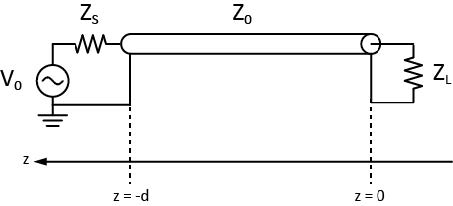
\includegraphics[width=\textwidth-7cm]{images/problem1.jpg}
\end{figure}

Voltage source generates 10 Ghz sine with 10V amplitude.

Tline terminated with $Z_L = 80 - 40j \Omega$, and $Z_0 = 100\Omega$. $\epsilon_{eff} = 4$ and $d = 22.5$ mm.

\begin{enumerate}
	\item Find the reflection coefficient at the load (z = 0) and at the source (z = -d)
	
	At the load:
	
	\begin{align*}
		\rho_L &= \frac{Z_L - Z_0}{Z_L + Z_0} \\
		\rho_L &= -0.0588 - 0.23539j \\
		|\rho_L| &= 0.242
	\end{align*}
	
	At any point on the line, we can derive an effective generalized $\rho(z)$ which represents the ratio of the backwards and forward traveling waves at a given point on the tline.
	
	\begin{align*}
		V(z) &= V_0^+ (e^{-j \beta z} + \rho_L e^{-j \beta z}) \\
		\rho(z) &= \frac{V_0^+ \rho_L e^{j \beta z}}{V_0^+ e^{-j \beta z}} \\
		\rho(z) &= \rho_L e^{2j \beta z}
	\end{align*}
	
	Notice that since $\beta = 2\pi / \lambda$, $\rho(z)$ repeats every $\lambda / 2$ traversed along the tline back to the generator. We can find $c_p$ and $\lambda$ for this tline and frequency.
	
	\begin{align*}
		c_p &= \frac{c_0}{\sqrt{\epsilon_{eff}}} \approx 1.5e8 \text{ m/s} \\
		\lambda &= \frac{c_p}{f} = 0.015 \text{ m} \\
		d / \lambda = 1.5 = 3 \cdot \frac{1}{2} \lambda \\
	\end{align*}
	
	So, $\rho(z)$ at $z = -d$ is $rho_L = 0.242$.
	
	\item Find the input impedance at the source (z = -d) and at z = 18.75mm.
	
	The general form is:
	
	\begin{align*}
		Z_{in}(-l) &= Z_0 \frac{Z_L + j Z_0 \tan(\beta l)}{Z_0 + j Z_L \tan(\beta l)} \\
		\beta &= \frac{2 \pi}{\lambda} = 418.879 \\
		Z_{in}(0) &= Z_L = 100 \Omega \\
		Z_{in}(-18.75 \text{ mm}) &= Z_{in}(\lambda + \lambda / 4) = \frac{Z_0^2}{Z_L} = 100 + 50j \\
	\end{align*}
	
	\item Plot the magnitude of the voltage along the line. Find voltage maximum, minimum, and SWR.
	
	We assume that $Z_S$ = $Z_0$:
	
	\begin{align*}
		SWR &= \frac{V_{max}}{V_{min}} = \frac{1 + |\rho_L|}{1 - |\rho_L|} \\
		SWR &= 1.64 \\
		V^+ &= \frac{Z_0}{Z_0 + Z_S} = 5 \text{ V} \\
		V_{max} &= |V^+| (1 + |\rho_L|) = 6.2 \text{ V} \\
		V_{min} &= |V^+| (1 - |\rho_L|) = 3.8 \text{ V} 
	\end{align*}
	
	Plot of voltage magnitude along line:
	\begin{figure}[H]
		\centering 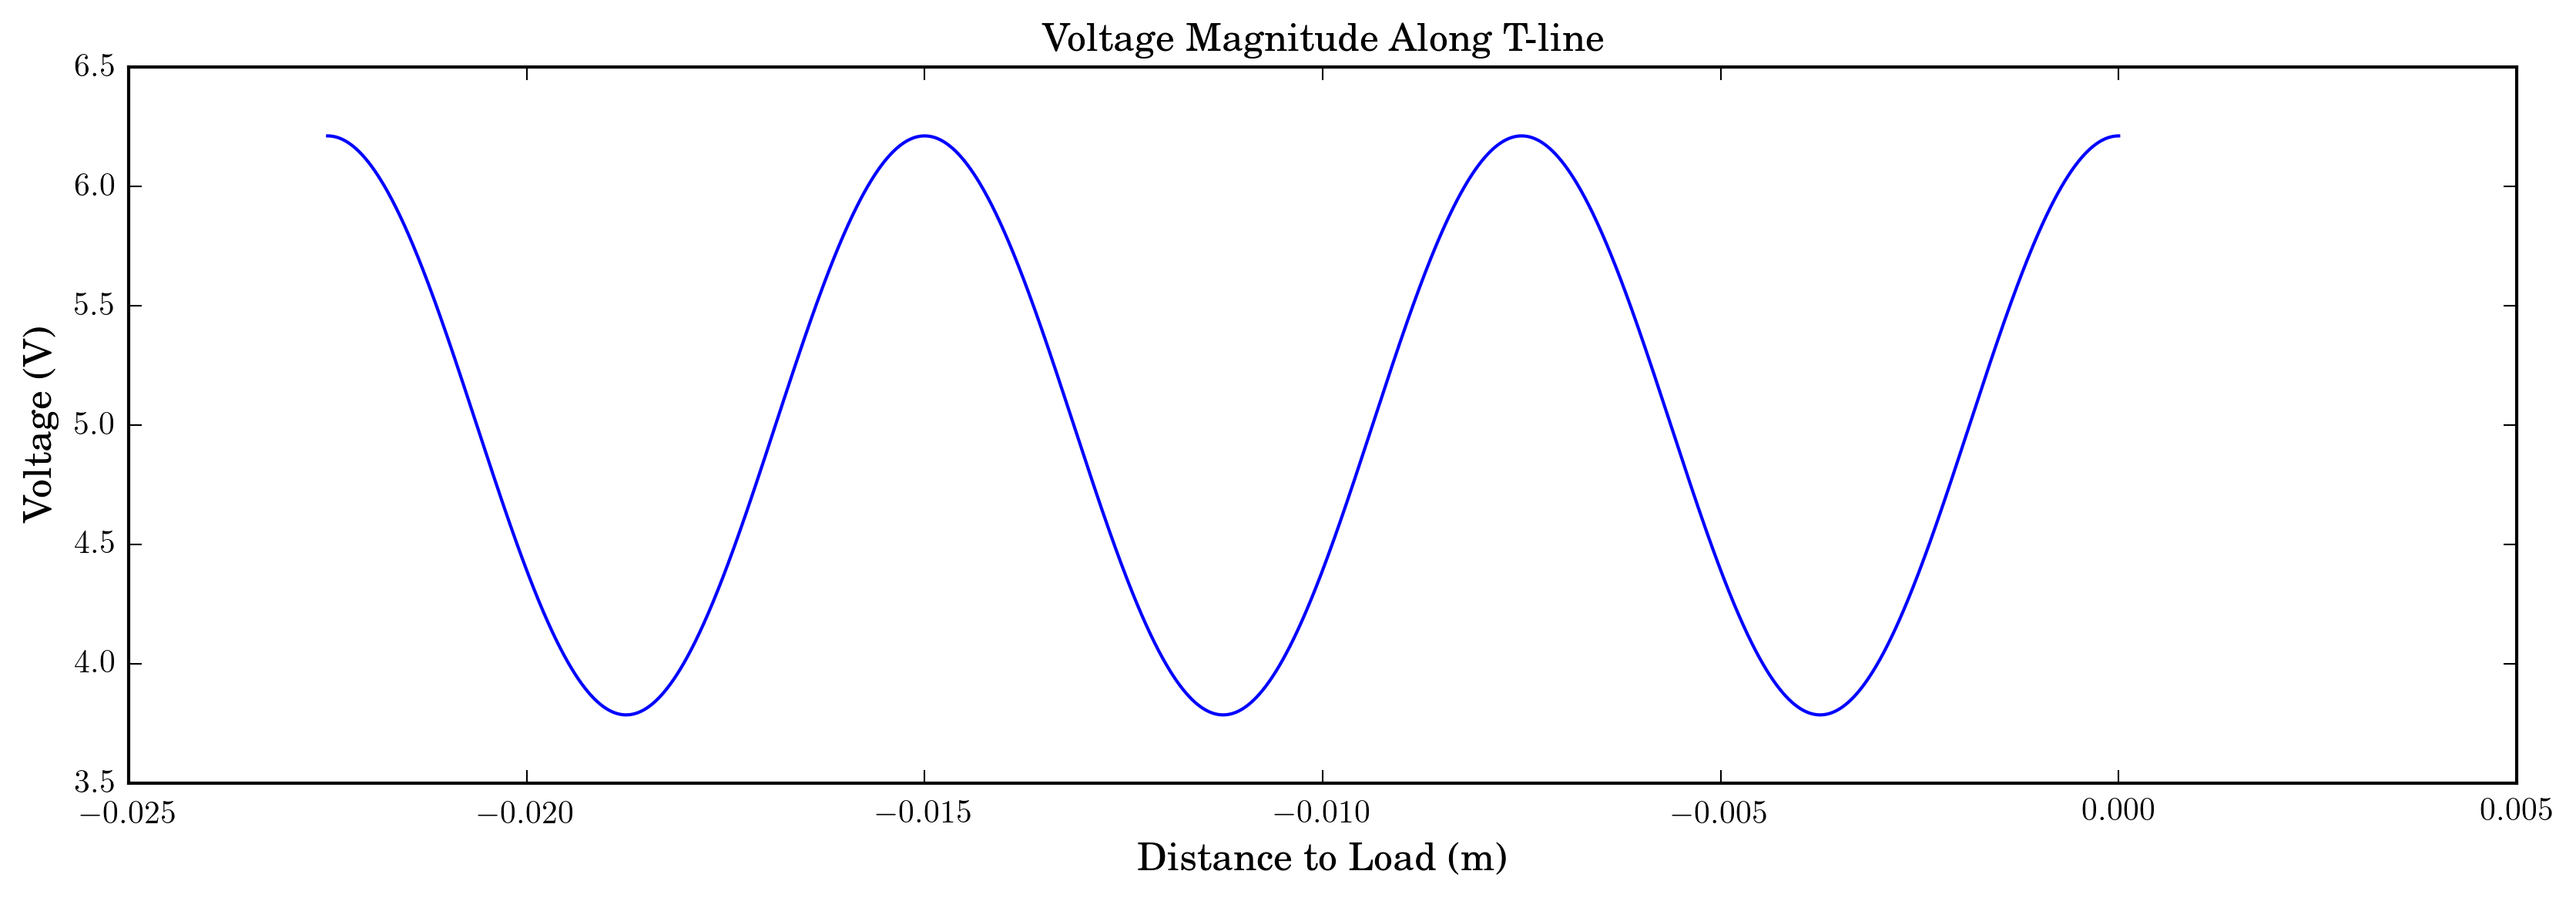
\includegraphics[width=\textwidth]{images/problem1.png}
	\end{figure}
\end{enumerate}

\section{T-Line Modeling}
We will derive an equivalent two-port circuit model for a short section of transmission line ($l << \lambda$) including loss.

\begin{enumerate}
	\item For a "pi" equivalent circuit shown below, find the two-port Z matrix.
	\begin{figure}[H]
		\centering 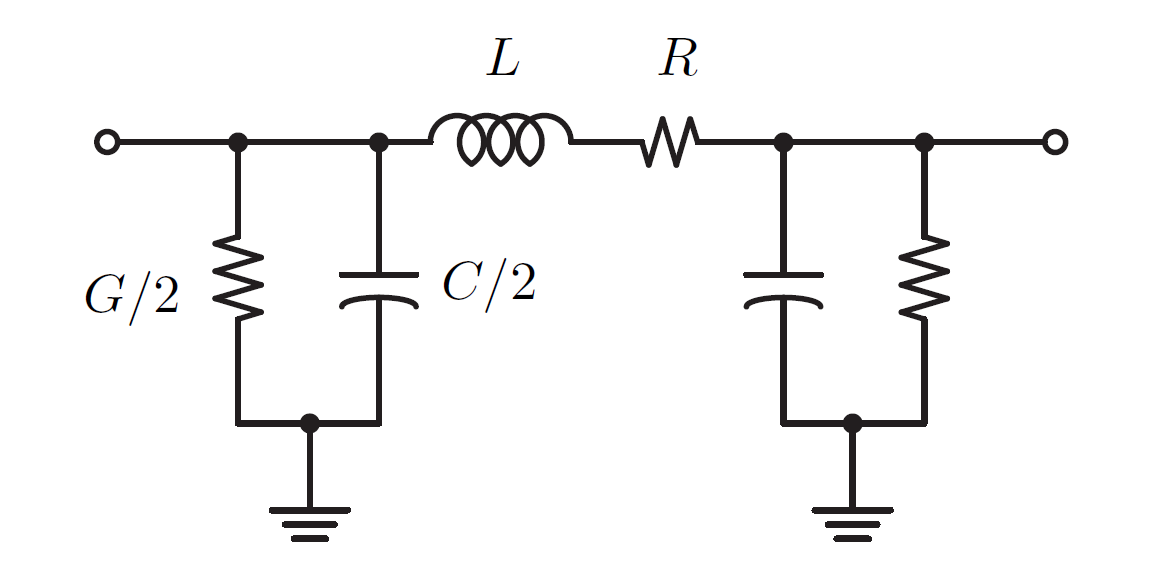
\includegraphics[width=\textwidth-6cm]{images/problem2_pi_network.png}
	\end{figure}

	Let's call the current flowing \emph{into} node 1 $i_1$ and the current flowing \emph{into} node 2 $i_2$. The voltage applied across node is is $v_1$ and $v_2$ for node 2. We will call each section of the pi network $Z_1, Z_2, Z_3$ going left to right and $Z_1 = Z_3$.
	
	\begin{align*}
		Z_{11} &= \frac{v_1}{i_1} \bigg\rvert_{i_2 = 0} = (Z_1 || (Z_2 + Z_3)) = \frac{Z_1(Z_2 + Z_3)}{Z_1 + Z_2 + Z_3} \\
		Z_{22} &= Z_{11} \text{ due to symmetry} \\
		Z_{12} &= \frac{v_1}{i_2} \bigg\rvert_{i_1 = 0} = \frac{Z_1 Z_3}{Z_1 + Z_2 + Z_3} \\
		Z_{21} &= Z_{12} \text{ due to reciprocity}
	\end{align*}
	
	\begin{align*}
		Z_1 = Z_3 &= \frac{2}{2j \omega C + G} \\
		Z_2 &= R + j \omega L
	\end{align*}
	
	\item Consider a section of transmission line with loss. Find the two port Z matrix. Use the transmission line impedance equation (general expression with loss).
	
	We begin with the general form using $\rho_L$:
	
	\begin{align*}
		Z_{in}(-l) &= \frac{V(-l)}{I(-l)} = Z_0 \frac{1 + \rho_L e^{-2 \gamma l}}{1 - \rho_L e^{-2 \gamma l}} \\
		\rho_L &= \frac{Z_L - Z_0}{Z_L + Z_0} \\
		Z_{in}(-l) &= Z_0 \frac{Z_L(1 + e^{-2 \gamma l}) + Z_0(1 - e^{-2 \gamma l})}{Z_0(1 + e^{-2 \gamma l}) + Z_L(1 - e^{-2 \gamma l})} \\
		Z_{in}(-l) &= Z_0 \frac{Z_L + Z_0 \tanh(\gamma l)}{Z_0 + Z_L \tanh(\gamma l)} \\
		\gamma &= \sqrt{(R + j \omega L)(G + j \omega C)} = \alpha + j \beta
	\end{align*}
	
	Now we open and short the transmission line to measure its Z parameters.
	
	\begin{align*}
		Z_{11} &= \frac{v_1}{i_1} \bigg\rvert_{i_2 = 0, Z_L = \infty} = Z_0 \frac{1}{\tanh(\gamma l)} \\
		Z_{22} &= Z_{11} \text{ due to symmetry} \\
		Z_{12} &= \frac{v_1}{i_2} \bigg\rvert_{i_1 = 0, Z_L = 0} = Z_0 \frac{1}{\sinh(\gamma l)} \\
		Z_{21} &= Z_{12} \text{ due to reciprocity}
	\end{align*}
	
	Keeping in mind that for a shorted tline, the voltage and current at a given point along the line are:
	
	\begin{align*}
		v(z) &= V^+ (e^{-\gamma z} + e^{\gamma z}) \\
		i(z) &= \frac{V^+}{Z_0} (e^{-\gamma z} - e^{\gamma z})
	\end{align*}
	
	\item Take the limit of a very short line and simplify the answer (Hint: use a Taylor series expansion and keep only the first few terms).
	
	Use the expansions:
	
	\begin{align*}
		\tanh(x) &= x - \frac{x^3}{3} + \frac{2x^5}{15} - ... \text{ for } |x| < \frac{\pi}{2} \\
		\sinh(x) &= x + \frac{x^3}{3!} + \frac{x^5}{5!} + ... \text{ for all x}
	\end{align*}
	
	We plug the first two terms into the t-line's Z matrix for $\tanh$ and $\sinh$. There isn't any other obvious simplification or limit taking to be done. 
	
	\item Using the previous results, now derive the values for L, R, C, and G for the equivalent circuit.
	
	I began this problem by equating the $Z_{11}$ and $Z_{12}$ parameters for the pi network and the transmission line. I also wrote down the equation relating $\gamma$ and $Z_0$ with R,G,L,C. 
	
	\begin{minted}{matlab}
%%
syms C w G R L
syms Z0 gamma l

Z1 = ((2/G)*(1/1i*w*C) / ((2/G) + (1/1i*w*C)));
%Z1 = 2 / (2*1i*w*C + G);
Z3 = Z1;
Z2 = R + 1i*w*L;

%%
Z_11 = (Z1*(Z2 + Z3)) / (Z1 + Z2 + Z3);
Z_12 = (Z1 * Z3) / (Z1 + Z2 + Z3);

Z_11_tline = Z0 / ((gamma*l - (gamma*l)^3 / 3 + 2*(gamma*l)^5 / 15));
Z_12_tline = Z0 / ((gamma*l + (gamma*l)^3 / 3*2 + (gamma*l)^5 / 5*4*3*2));

gamma_RLGC_relation = gamma == sqrt((R + 1i*w*L) * (G + 1i*w*C));
Z0_LC_relation = Z0 == sqrt((R + 1i*w*L)/(G + 1i*w*C));

sol = solve([Z_11 == Z_11_tline, Z_12 == Z_12_tline], [R, G, L, C]);
	\end{minted}
	
	I tried to give different permutations of these equations to the solver, but wasn't able to find any sensible solution for R, G, L, C in terms of $Z_0$, $\gamma$, and $\omega$ although I'm sure one exists.

\end{enumerate}

\section{Impedance Matching for Maximum Power Delivery}

\begin{enumerate}
	\item What is the maximum power that can be extracted from the source shown below? What is the optimal load impedance for the maximum power delivery to happen?
		\begin{figure}[H]
		\centering 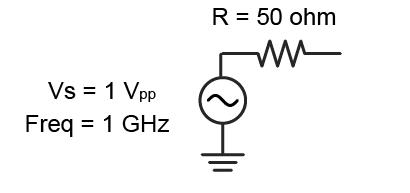
\includegraphics[width=\textwidth-10cm]{images/problem3a.jpg}
	\end{figure}
	
	\begin{align*}
		|I_{s}| &= \frac{|V_s|}{|R_s + R_L|} \\
		I_{s,rms} &= \frac{1}{2} |I_{s}| \\
		V_{L} &= I_{s,rms} R_L \\
		P_{L} &= I_{s,rms} V_L = I_{s,rms}^2 R_L = 1/2 (\frac{V_s}{R_s + R_L})^2 R_L \\
		\frac{\partial P_L}{\partial R_L} &= (\frac{-R_s}{R_L})^2 + 1
	\end{align*}
	
	Setting the denominator of derivative to 0 and solving gives $R_L = \pm R_s \rightarrow R_L = R_s$. Indeed, this minimizes the denominator, and thus maximizes the power delivered to the load.
	
	\begin{align*}
		P_{max} = \frac{V_s^2}{8 R_L} = 2.5 \text{ mW}
	\end{align*}
	
	\item Use this source to drive a $500\Omega$ load and we directly connect the load to the source, as illustrated by the figure below. What is the power delivered to the $500 \Omega$ load and the load voltage?
	
	\begin{figure}[H]
		\centering 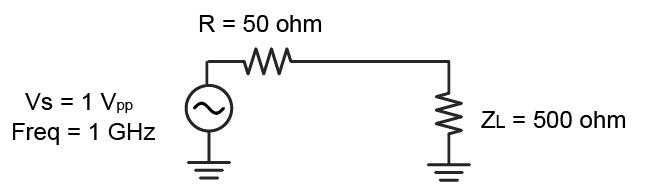
\includegraphics[width=\textwidth-8cm]{images/problem3b.jpg}
	\end{figure}

	\begin{align*}
		P_L = 0.8 \text{ mW} \\
		V_L = I_{s,rms} R_L = 0.45 \text{ V}
	\end{align*}
	
	\item Let's try to achieve impedance matching by putting a quarter-wavelength transmission line between the load and source, as indicated by the below figure. Find the characteristic impedance $Z_0$ that maximizes the power delivered to the load. What are the corresponding power and voltage at the load?
	
	\begin{figure}[H]
		\centering 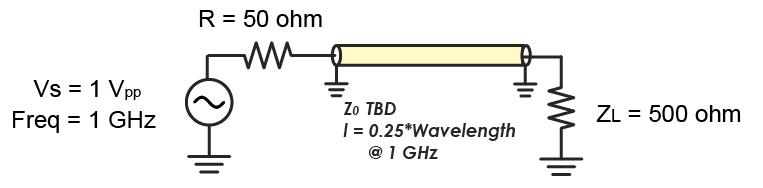
\includegraphics[width=\textwidth-6cm]{images/problem3c.jpg}
	\end{figure}

	The general form of input impedance for a lossless tline is:
	
	\begin{align*}
		Z_{in}(-l) &= Z_0 \frac{Z_L + j Z_0 \tan(\beta l)}{Z_0 + j Z_L \tan(\beta l)} \\
		Z_{in}(-\lambda/4) &= \frac{Z_0^2}{Z_L} = 50 \rightarrow Z_0 = 158 \Omega \\
		P_{L} &= P_{max} = 2.5 mW \text{ since the tline is lossless} \\
		V_{L} &= \sqrt{P_L R_L} = 1.118 \text{ V}
	\end{align*}
	
	\item Following part c) assume the source frequency can change, what is the frequency interval where the power delivered to the $500\Omega$ load is less than 3 dB from the maximum value? Use ADS to verify.
	
	Assume that $\epsilon_{eff} = 4$. -3 dB power reduction is equivalent to the power halving. We fix the transmission line's length and $Z_0$ and sweep $\beta$ to find where the effective resistance looking into the transmission line becomes sufficiently high to halve power.
	
	\begin{align*}
		P_L' &= 1/2 (\frac{1}{50 + R_L})^2 R_L = 2.5 /2 \text{ mW} \\
		\text{Solving: } R_L &= 292 \Omega \\
		\beta &= 76.1 \text{ to get an effective } R_L \text{ of } 292 \Omega  \\
		&\rightarrow f' = 1.8 \text{ Ghz}
	\end{align*}
	
	In ADS:
	
	\begin{figure}[H]
		\centering 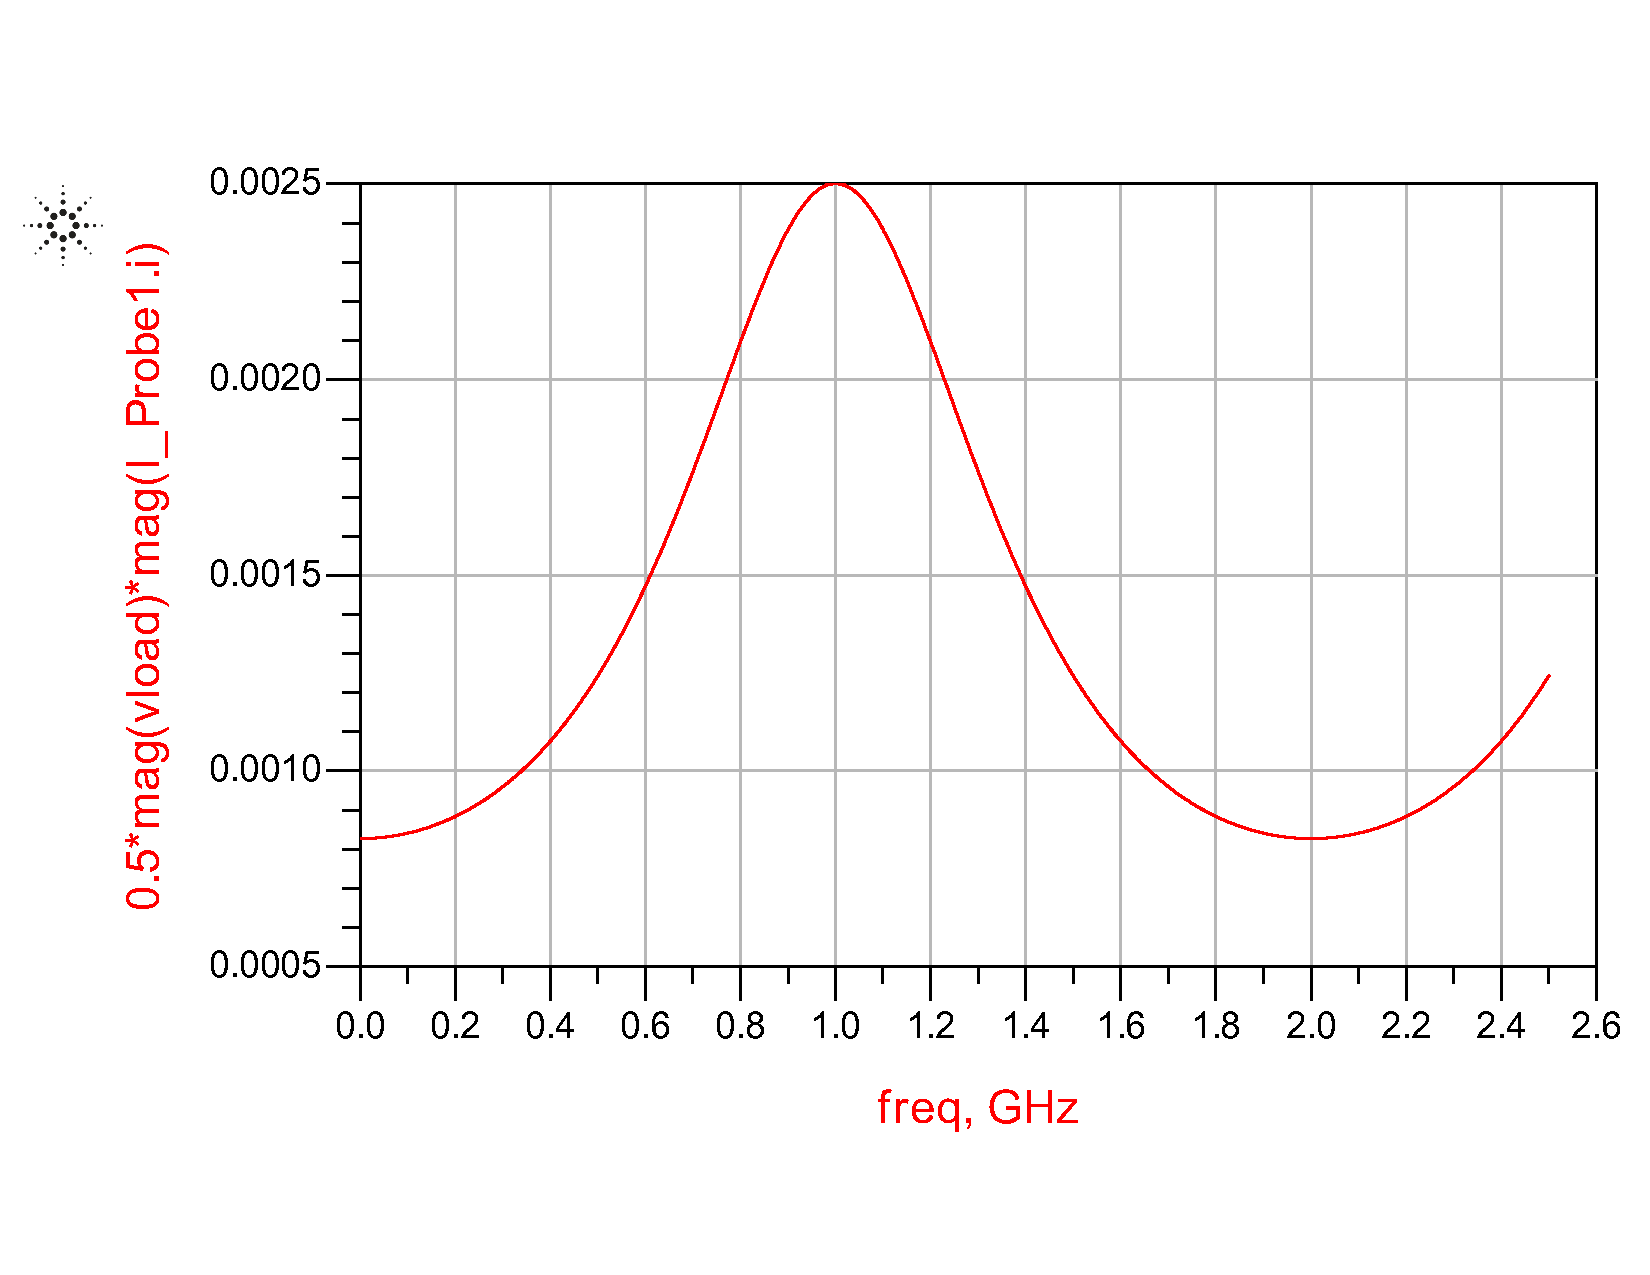
\includegraphics[width=\textwidth-4cm]{images/problem3d.pdf}
	\end{figure}

	The simulation indicates a power halving at around 1.5 Ghz. I suspect my assumption about $\epsilon_{eff}$ was problematic in the hand calculation.
\end{enumerate}

\end{document}
